\documentclass[11pt]{report}

% Paquetes y configuraciones adicionales
\usepackage{graphicx}
\usepackage[export]{adjustbox}
\usepackage{caption}
\usepackage{float}
\usepackage{titlesec}
\usepackage{geometry}
\usepackage[hidelinks]{hyperref}
\usepackage{titling}
\usepackage{titlesec}
\usepackage{parskip}
\usepackage{wasysym}
\usepackage{tikzsymbols}
\usepackage{fancyvrb}
\usepackage{xurl}
\usepackage{hyperref}
\usepackage[spanish]{babel}
\usepackage{listings}
\usepackage{subcaption}
\usepackage{xcolor}

\newcommand{\subtitle}[1]{
  \posttitle{
    \par\end{center}
    \begin{center}\large#1\end{center}
    \vskip0.5em}
}

% Configura los márgenes
\geometry{
  left=2cm,   % Ajusta este valor al margen izquierdo deseado
  right=2cm,  % Ajusta este valor al margen derecho deseado
  top=3cm,
  bottom=3cm,
}

% Configuración de los títulos de las secciones
\titlespacing{\section}{0pt}{\parskip}{\parskip}
\titlespacing{\subsection}{0pt}{\parskip}{\parskip}
\titlespacing{\subsubsection}{0pt}{\parskip}{\parskip}

% Redefinir el formato de los capítulos y añadir un punto después del número
\makeatletter
\renewcommand{\@makechapterhead}[1]{%
  \vspace*{0\p@} % Ajusta este valor para el espaciado deseado antes del título del capítulo
  {\parindent \z@ \raggedright \normalfont
    \ifnum \c@secnumdepth >\m@ne
        \huge\bfseries \thechapter.\ % Añade un punto después del número
    \fi
    \interlinepenalty\@M
    #1\par\nobreak
    \vspace{10pt} % Ajusta este valor para el espacio deseado después del título del capítulo
  }}
\makeatother

% Configura para que cada \chapter no comience en una pagina nueva
\makeatletter
\renewcommand\chapter{\@startsection{chapter}{0}{\z@}%
    {-3.5ex \@plus -1ex \@minus -.2ex}%
    {2.3ex \@plus.2ex}%
    {\normalfont\Large\bfseries}}
\makeatother

% Configurar los colores para el código
\definecolor{codegreen}{rgb}{0,0.6,0}
\definecolor{codegray}{rgb}{0.5,0.5,0.5}
\definecolor{codepurple}{rgb}{0.58,0,0.82}
\definecolor{backcolour}{rgb}{0.95,0.95,0.92}

% Configurar el estilo para el código
\lstdefinestyle{mystyle}{
  backgroundcolor=\color{backcolour},   
  commentstyle=\color{codegreen},
  keywordstyle=\color{magenta},
  numberstyle=\tiny\color{codegray},
  stringstyle=\color{codepurple},
  basicstyle=\ttfamily\footnotesize,
  breakatwhitespace=false,         
  breaklines=true,                 
  captionpos=b,                    
  keepspaces=true,                 
  numbers=left,                    
  numbersep=5pt,                  
  showspaces=false,                
  showstringspaces=false,
  showtabs=false,                  
  tabsize=2
}

%==============================================================================
% Cosas para la documentación LateX
% % Sangría
% \setlength{\parindent}{1em}Texto

% % Quitar sangría
% \noindent

% % Punto
% \CIRCLE \ \ \textbf{Texto} \emph{algo}
% \begin{itemize}
%   \item \textbf{Negrita:} Texto
%   \item \textbf{Negrita:} Texto
% \end{itemize}

% % Introducir código
% \begin{center}
%   \begin{BVerbatim}
%     ... Código
%   \end{BVerbatim}
% \end{center}

% Poner una imagen
% \begin{figure}[H]
%   \centering
%   \includegraphics[scale=0.55]{img/}
%   \caption{Exportación de la base de datos en formato sql}
%   \label{fig:exportación de la base de datos en formato sql}
% \end{figure}

% Poner dos imágenes
% \begin{figure}[H]
%   \begin{subfigure}{0.5\textwidth}
%     \centering
%     \includegraphics[scale=0.45]{img/}
%     \caption{Texto imagen 1}
%   \end{subfigure}%
%   \begin{subfigure}{0.5\textwidth}
%     \centering
%     \includegraphics[scale=0.45]{img/}
%     \caption{Texto imagen 2}
%   \end{subfigure}
%   \caption{Texto general}
% \end{figure}

% % Poner una tabla
% \begin{table}[H]
%   \centering
%   \begin{tabular}{|c|c|c|c|}
%     \hline
%     \textbf{Campo 1} & \textbf{Campo 2} & \textbf{Campo 3} & \textbf{Campo 4} \\ \hline
%     Texto & Texto & Texto & Texto \\ \hline
%     Texto & Texto & Texto & Texto \\ \hline
%     Texto & Texto & Texto & Texto \\ \hline
%     Texto & Texto & Texto & Texto \\ \hline
%   \end{tabular}
%   \caption{Nombre de la tabla}
%   \label{tab:nombre de la tabla}
% \end{table}

% % Poner codigo de un lenguaje a partir de un archivo
% \lstset{style=mystyle}
% The next code will be directly imported from a file
% \lstinputlisting[language=Python]{code.py}

% “Texto entre comillas dobles”

%==============================================================================

\begin{document}

% Portada del informe
\title{Práctica 11. Hardening con \emph{SELinux} y \emph{AppArmor}}
\subtitle{Seguridad de Sistemas Informáticos}
\author{Carlos Pérez Fino, Cheuk Kelly Ng Pante \& Cristopher Manuel Afonso Mora}
\date{\today}

\maketitle

\pagestyle{empty} % Desactiva la numeración de página para el índice

% Índice
\tableofcontents

% Nueva página
\cleardoublepage

\pagestyle{plain} % Vuelve a activar la numeración de página
\setcounter{page}{1} % Reinicia el contador de página a 1

% Secciones del informe
% Capitulo 1
\chapter{Instalación de las máquinas virtuales}
Para esta práctica se va a instalar dos máquinas virtuales, una \emph{Ubuntu Server 16.04} 
y una \emph{CentOS 7} para estudiar las configuraciones de hardening del sistema operativo
basados en un control de acceso MAC implementadas en estos sistemas con \emph{AppArmor} 
y \emph{SELinux} respectivamente.

\begin{figure}[H]
  \centering
  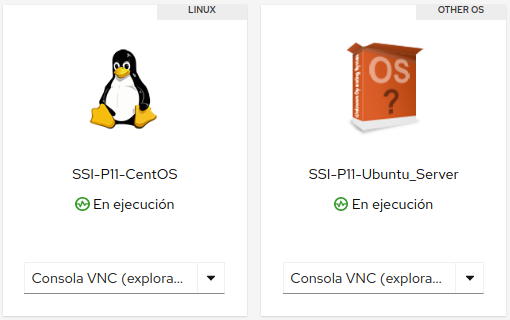
\includegraphics[scale=0.45]{img/mv_instalation.png}
  \caption{Instalación de las máquinas virtuales}
\end{figure}

% Capitulo 2
\chapter{Instalación y configuración de apache para la aplicación vulnerable \emph{DVWA}}
\section{Instalación en Ubuntu Server 16.04}
El primer paso es, antes de instalar Damn Vulnerable Web Application (DVWA) en la máquina virtual de Ubuntu Server 16.04,
es instalar el servidor web Apache, el gestor de base de datos MariaDB y PHP. Para ello, ejecutamos
los siguientes comandos:
\begin{verbatim}
$ sudo apt-get update
$ sudo apt-get install -y apache2 libapache2-mod-php
$ sudo apt-get install -y mariadb-server mariadb-client 
$ sudo apt-get install -y php php-mysqli php-gd 
\end{verbatim}

Una vez instalado los paquetes, vamos a inicializar el servicio de Apache con el siguiente comando:
\begin{BVerbatim}
sudo service apache2 start
\end{BVerbatim}

y a ejecutar el script de configuración de MariaDB con el siguiente comando:
\begin{BVerbatim}
sudo mysql_secure_installation
\end{BVerbatim}

Y ahora vamos a instalar DVWA descargandolo desde el repositorio oficial de DVWA en GitHub. Para ello, primero instalamos git y clonamos el repositorio de DVWA en el directorio
\emph{/var/www/html}. Lo pasos de Instalación son los siguientes:
\begin{verbatim}
$ sudo apt-get install git
$ git clone https://github.com/digininja/DVWA.git
$ sudo mv DVWA/ /var/www/html/
\end{verbatim}

\section{Instalación en CentOS 7}
Para instalar DVWA en CentOS 7, primero instalamos el servidor web Apache, el gestor de base de datos MariaDB y PHP. Para ello, ejecutamos
los siguientes comandos:
\begin{verbatim}
$ sudo yum update
$ sudo yum install -y httpd mariadb-server mariadb php php-mysql php-gd
\end{verbatim}

Una vez instalado los paquetes, vamos a inicializar el servicio de Apache con el siguiente comando:
\begin{BVerbatim}
sudo systemctl start httpd.service
\end{BVerbatim}

y a ejecutar el script de configuración de MariaDB con el siguiente comando:
\begin{BVerbatim}
sudo mysql_secure_installation
\end{BVerbatim}

Y ahora vamos a instalar DVWA descargandolo desde el repositorio oficial de DVWA en GitHub. Para ello, primero instalamos git y clonamos el repositorio de DVWA en el directorio
\emph{/var/www/html}. Lo pasos de Instalación son los siguientes:
\begin{verbatim}
$ sudo yum install git
$ git clone https://github.com/digininja/DVWA.git
$ sudo mv DVWA/ /var/www/html/
\end{verbatim}

\section{Configuración de DVWA}
Para empezar la configuración de DVWA se va a acceder al directorio \emph{/var/www/html/DVWA} y copiamos el archivo \emph{config.inc.php.dist} a
\emph{config.inc.php} con el siguiente comando:
\begin{verbatim}
$ sudo cp config/config.inc.php.dist config/config.inc.php
\end{verbatim}

Ahora, vamos a configurar las variables de configuración de DVWA en el archivo \emph{config.inc.php}. Para ello, ejecutamos el siguiente comando:
\begin{verbatim}
$_DVWA[ 'db_server' ]   = getenv('DB_SERVER') ?: '127.0.0.1';
$_DVWA[ 'db_database' ] = 'dvwa';
$_DVWA[ 'db_user' ]     = 'dvwa';
$_DVWA[ 'db_password' ] = 'ssi12345';
$_DVWA[ 'db_port' ]      = '3306';
\end{verbatim}

Y ahora vamos a crear la base de datos \emph{dvwa} y el usuario \emph{dvwa} con el siguiente comando:
\begin{verbatim}
$ sudo mysql -u root -p
mysql> create database dvwa;
Query OK, 1 row affected (0.00 sec)

mysql> create user dvwa@localhost identified by 'ssi12345';
Query OK, 0 rows affected (0.01 sec)

mysql> grant all on dvwa.* to dvwa@localhost;
Query OK, 0 rows affected (0.01 sec)

mysql> flush privileges;
Query OK, 0 rows affected (0.00 sec)
\end{verbatim}



\chapter{Bibliografía} % En formato APA
\begin{enumerate}
\item Ng Pante, C. (2001). Titulo. Nombre pagina web. Recuperado de \url{http://url.com}

\end{enumerate}

\end{document}